\documentclass[10pt]{article}
\usepackage{arxiv}
\usepackage[T1]{fontenc}
\usepackage[utf8]{inputenc}
\usepackage{amsmath,amssymb,amsthm}
\usepackage{booktabs,array,tabularx,longtable}
\usepackage{graphicx,microtype}
\usepackage{enumitem}
\usepackage[numbers,sort&compress]{natbib}
\usepackage{xcolor}
\usepackage[hidelinks]{hyperref}
\hypersetup{pdftitle={NeuroCAD: An Auditable Bounded CAD Compiler and Constraint-Evidence System},pdfauthor={Ryan Gomez, The Bu1LD},pdfsubject={Current-evidence research manuscript; bounded compiler and synthetic constraint-receipt evidence}}
\usepackage{url,placeins,fancyvrb,needspace}
\usepackage{tikz}
\usetikzlibrary{arrows.meta,positioning}
\renewcommand{\shorttitle}{\footnotesize NeuroCAD: bounded compilation and evidence}
\renewcommand{\headeright}{Evidence synthesis}
\renewcommand{\undertitle}{Current-evidence research manuscript}
\newcommand{\code}[1]{\texttt{\detokenize{#1}}}
\newcommand{\ind}{\mathbb{1}}
\newcommand{\Hsh}{\operatorname{SHA256}}
\newcommand{\canon}{\operatorname{canonicalJSON}}
\newcolumntype{Y}{>{\raggedright\arraybackslash}X}
\newtheorem{proposition}{Proposition}
\setlist{itemsep=2pt,topsep=3pt,leftmargin=1.5em}
\setlength{\emergencystretch}{2em}
\title{NeuroCAD: An Auditable Bounded CAD Compiler\\and Constraint-Evidence System}
\author{Ryan Gomez\\The Bu1LD}
\date{22 October 2026}

\begin{document}
\maketitle
\begin{abstract}
Computer-aided design automation requires distinctions among syntactic validity,
geometric validity, conformity to stated intent, and physical adequacy. NeuroCAD
is a deterministic bounded compiler and analytical-evidence system that makes
these distinctions explicit. Its pipeline converts supported dimensioned text
into a typed constructive-solid-geometry program, checks declared constraints,
exports executable geometry, and retains source and artifact identities.
A separate receipt mechanism binds analytical requests to canonical component
geometry, explicit material declarations, and named loads. We consolidate the
existing implementation, specifications, and retained evidence without
reopening completed studies. The source-bound controlled compiler run contains
240/240 exact semantic matches, 1,000/1,000 static program checks, and 240/240
fresh kernel executions; its generated grammar and simple baselines limit
interpretation. A separately frozen 216-case synthetic physics-receipt study
accepted 48/48 valid requests, detected 96/96 declared contradictions or stale
expected hashes, and detected 48/48 later geometry changes. A hash-only
ablation detected later changes but missed all 72 semantic contradictions.
One internal Linux repetition reproduced all 13 endpoint counts on the same
216 cases, without adding independent confirmation.
These are positive software-contract results, not evidence of physical
accuracy or general language understanding. An archival audit finds 1,211 of
1,212 listed compiler artifacts present with matching hashes; one original
log is missing. We also disclose timing-digest and median-definition issues,
preserve the falsified historical typed-parser claim, and distinguish later
engineering extensions from confirmation. The original compiler study remains
mixed; the receipt study is supported within its controlled contract.
Independent language, physical-fit, and user studies remain unexecuted.
\end{abstract}
\keywords{parametric CAD \and deterministic compilation \and provenance
\and conformance testing \and research reproducibility}

\section{Introduction}

A useful CAD assistant must do more than produce a plausible rendering. A
request such as a dimensioned plate with a specified hole pattern concerns
editable parameters, feature counts, spatial relations, and permissible
failures. A script can execute while describing the wrong part. A closed mesh
can omit a requested hole. A correct formula can use a dimension that no longer
matches the design. These are different failure modes and require different
evidence.

NeuroCAD addresses a deliberately restricted version of this problem. Its
supported research method is a deterministic text-to-CAD compiler, not a
trained neural model. Supported prompts are mapped to an explicit intermediate
representation (IR), checked, serialized, and exported. Unsupported or
incomplete requests produce errors. A separately versioned analytical layer
returns calculations together with their assumptions and dependency receipts.
The point of the restriction is that the admitted behavior can be specified
and inspected; it does not establish competence outside that restriction.

This manuscript has two scientific objectives. First, it describes exactly
what existing controlled compiler evidence demonstrates. Second, it reports a
completed synthetic study of a narrow dependency-binding mechanism. The latter
asks whether semantic agreement checks and geometry freshness checks detect
predeclared contradictory or stale analytical requests while accepting valid
ones. The central mechanism is explicit dependency comparison: a hash tracks
declared content identity, while separate numeric comparisons detect selected
cross-field contradictions. Neither mechanism evaluates the physical truth of
an assumption.

The repository already contains distinct scientific histories. The original
typed-parser causal claim was falsified and is not rehabilitated by later
compiler repairs. The compiler research line has a terminal \emph{mixed}
disposition. Physics v2 has a separate completed 216-case controlled result,
now accompanied by one explicitly internal execution on another environment.
Physics v3 adds engineering functionality and regression evidence, including
retained failures and separately versioned repairs. This manuscript preserves
these histories. It is a current-evidence synthesis and technical report, not
a retrospective preregistration of a new joint experiment.

Our contributions are correspondingly bounded: (i) an explicit specification
of the evaluated deterministic compiler and analytical receipt mechanisms;
(ii) an evidence-qualified account of their controlled results and ablations;
(iii) a claim-to-artifact map, reusable table/figure regeneration, and an
archival audit that discloses missing evidence; and (iv) a precise separation
between implementation correctness, measured conformance, and external
validation. We claim neither a new general CAD learning algorithm nor
state-of-the-art text-to-CAD performance.

\section{Related work and novelty boundary}

\paragraph{Executable and parametric CAD generation.}
DeepCAD models CAD construction sequences with a Transformer
\citep{wu2021deepcad}. Text2CAD generates parametric sequences from textual
instructions \citep{khan2024text2cad}. CAD-Recode produces executable Python
CAD from point clouds \citep{rukhovich2025cadrecode}; its input modality differs
from NeuroCAD's text interface. CAD-Coder by Guan et al.\ generates CadQuery
programs using supervised training, geometric rewards, and planning
\citep{guan2025cadcoder}. These works already establish programmatic,
editable representations and language-conditioned CAD. They are relevant
prior art, not measured baselines in the retained NeuroCAD experiments.

\paragraph{Intent, constraints, and evaluation.}
ExpConCAD addresses omitted spatial constraints using construction-aware
reasoning and retrieved experience \citep{liu2026expconcad}. CIT-CAD makes an
intent tree guide both code generation and constraint verification, then uses
mismatches to localize repair \citep{du2026citcad}. Thus an explicit intent
representation followed by checking and repair is not, by itself, a new
contribution. CADTests evaluates prompt requirements directly on generated
B-reps and uses mutation-refined tests for evaluation and generation feedback
\citep{mallis2026cadtests}. HistCAD evaluates whether constraint predictions
support specified dimensional edits while preserving other relations and
rebuilding the complete history \citep{dong2026histcad}. Initial geometry
validity therefore cannot substitute for editability or requirement fidelity.
PICARD provides an earlier example of constraining formal-language generation
through incremental parsing \citep{scholak2021picard}, although its demonstrated
task is SQL rather than CAD.

\paragraph{Provenance and geometry validity.}
The W3C PROV data model already represents entities, activities, derivations,
and responsible agents \citep{moreau2013prov}. RO-Crate describes packaging
research objects with contextual metadata \citep{rocrate2025}. NeuroCAD does
not claim to invent hashing, provenance, digital-thread traceability, or CAD/CAE
associativity, and this package is not asserted to be RO-Crate conformant.
Open CASCADE's shape analyzer checks specified geometric and topological
consistency conditions \citep{occt2026}. Those checks are useful within their
defined scope; they do not establish correspondence to a user's intended
function.

\paragraph{Defensible comparison.}
The evaluated distinction is a bounded executable contract and its observed
implementation behavior. The retained compiler comparators are intentionally
simple reference points. Their performance cannot support superiority to
Text2CAD, CAD-Coder, CIT-CAD, or an equally capable human CAD workflow.
Similarly, adding a freshness mechanism to an arm that lacks one shows a
mechanism contrast, not a discovery that provenance is beneficial in general.
No absence-of-prior-art claim is needed for the results reported here.

\section{Problem formulation and evidence levels}

Let \(x\) be a prompt and \(L\) the declared supported language. The compiler is
a partial deterministic map \(C:\mathcal X\to\mathcal P\cup\mathcal E\), where
\(\mathcal P\) contains canonical programs and \(\mathcal E\) explicit errors.
A valid reference signature \(y\) records the task's declared primitive,
dimensions, feature counts and sizes, and enclosure state where applicable.
The benchmark success indicator is
\begin{equation}
 s(x,y)=\ind[C(x)=p\in\mathcal P]\,
        \ind[V(p)=\mathrm{valid}]\,
        \ind[\sigma(p)\equiv_\epsilon y],
\end{equation}
where \(V\) is static validation, \(\sigma\) the frozen signature extractor,
and \(\equiv_\epsilon\) its numeric comparison (absolute tolerance
\(10^{-6}\) for the controlled signature fields). Dictionary comparison
requires the expected fields, rather than rejecting every extra predicted
field. This is exactness
over selected fields, not full geometric equivalence or complete design intent.

For an invalid or unsupported prompt, fail-closed success means that no
program is returned and an explicit failure is recorded. Acceptance and
rejection must be reported separately: a system that rejects every request
has no useful valid-input coverage. Repeated executions of one prompt are
determinism observations, not new independent experimental units.

\begin{table}[t]
\centering
\caption{Evidence levels are not interchangeable. A pass at one level does
not entail the next.}
\label{tab:levels}
\small
\begin{tabularx}{\linewidth}{p{0.22\linewidth}XX}
\toprule
Level & Observable question & Remaining uncertainty \\
\midrule
Static admission & Does the program satisfy schema, type, graph and declared
constraint checks? & Did the parser recover the intended part? \\
Kernel execution & Can the declared backend build a nonempty artifact? &
Does it meet all dimensional and topological requirements? \\
Requirement conformance & Do the frozen predicates or task fields pass? &
Are the predicates complete and independently correct? \\
Dependency freshness & Does recorded content still match its dependency? &
Was that dependency authoritative or physically appropriate? \\
Physical/user evidence & Does a measured part or observed workflow meet its
declared endpoint? & Generality beyond the measured conditions \\
\bottomrule
\end{tabularx}
\end{table}

The analytical task is separately defined. A request
\(R=(m,x_a,c)\) consists of a versioned model \(m\), finite explicitly named
inputs \(x_a\), and optional context \(c\). Evaluation produces an error or
\begin{equation}
Y=(m_v,x_a,y_a,A,B,H_R,H_x,c_{\mathrm{receipt}}),
\end{equation}
where \(y_a\) are analytical outputs, \(A\) assumptions, \(B\) a claim boundary,
and the hashes bind specified content. This record can be internally
consistent while using an inappropriate model or an inaccurate material card.

\section{Deterministic compiler specification}

\subsection{Language admission and representation}

The evaluated compiler accepts fully dimensioned plate, box, open-top
enclosure, cylinder, and sphere templates, including specified holes and slots.
It parses dimension sequences using \code{x}, a multiplication separator, or
\code{by}, and also named dimensions. Supported units normalize to millimetres:
millimetres, centimetres, metres, and inches use factors \(1,10,1000,25.4\).
Holes require their diameter, slots their two dimensions, and supported feature
counts are bounded. Unsupported domains and missing required quantities are
semantic errors. The study is not a claim that arbitrary English maps to these
templates correctly.

The original canonical representation is \code{neurocad-ir-v1}. It contains
uniquely identified primitive leaves, Boolean composition nodes, explicit
roots, and optional declared constraints. Leaves include box, planar-rounded
box, sphere, cylinder, cone, and torus; composition operations are union,
difference, and intersection. Nodes retain translation, XYZ rotation, scale,
and role. Supported constraint kinds include dimension, coincidence, offset,
child count, and bounds. This CSG representation is distinct from the later
experimental \code{neurocad-feature-ir-v0alpha1} history representation.

The latter admits feature records and semantic selectors for exact-backend
experimentation. A selector names an entity kind, generating feature,
predicates, optional role, and uniqueness requirement; it does not persist a
raw kernel face index as its stable identity. This representation's existence
does not imply that every listed feature has been validated on every backend.
The original compiler results are not scores for this later representation.

\subsection{Validation, construction, and serialization}

The forward process is: normalize the admitted text; parse task quantities and
features; construct the compatibility graph; adapt to canonical IR; validate;
serialize; export; optionally execute the selected kernel; independently read
the resulting artifact; then publish its verification record. Static validation
uses a Draft 2020-12 schema plus semantic checks for identifier uniqueness,
references, hierarchy, parameter domains, transformations, and declared
constraints. The original study limits programs to 1,024 nodes and depth 128;
structured input is capped at 1 MiB. These bounds limit resource exhaustion,
but do not prove parser complexity for every hostile string.

Finite numeric admission must distinguish a number from a Boolean or textual
number and must avoid overflow during conversion. In particular, Python's
Boolean subtype relation to integers is not an acceptable admission rule.
Canonical program round-trip identity is tested as \(P(S(p))=p\), with \(S\)
the deterministic serializer and \(P\) the parser. Graph validation visits
vertices and references, giving \(O(N+E)\) structural work under bounded-size
node fields; serialization and export also depend on output length. A bound
on IR size does not bound the runtime of an arbitrary geometry kernel.

For the historical executed geometry study, the exporter emits OpenSCAD CSG,
the kernel is OpenSCAD 2021.01, and tessellation uses \code{$fn=48}.
Execution uses a fixed argument vector, timeout, and nonempty output checks.
Retained artifacts are read through a separate mesh library and checked for
the specified volume/topology/extents conditions. Mesh checks do not turn the
output into exact B-rep geometry. Later STEP/BREP backends have separate
engineering evidence and do not retroactively change the historical study.

\subsection{Editable state and training status}

A parameter edit targets a named field, followed by validation, serialization,
reparse, and export. The retained edit experiment changes box width. It does
not establish robust topological naming for arbitrary feature histories or
designer usability. Later conversational edit and clarification behavior
belongs to the current engineering implementation.

There is no learned architecture, optimizer, training loss, gradient,
checkpoint, or training seed for the supported NeuroCAD method. These items
are inapplicable, rather than unfinished neural components. The retrieval
comparator indexes only train-labelled controlled prompts using token-set
Jaccard similarity and copies the nearest reference signature. Its label
access is reported explicitly.

\begin{figure}[t]
\centering
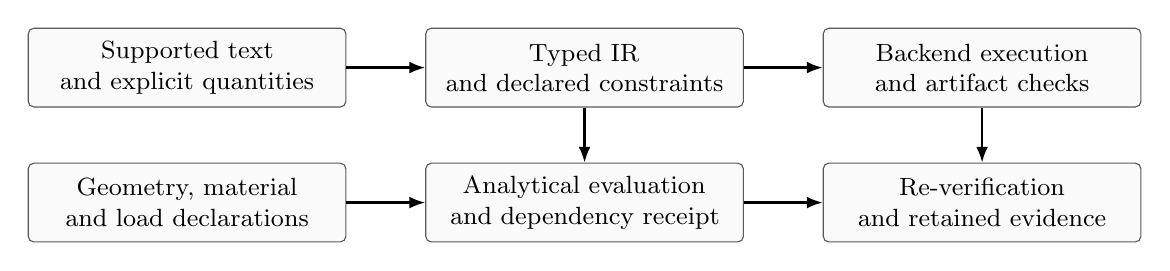
\begin{tikzpicture}[
 box/.style={draw=black!65,rounded corners=2pt,align=center,font=\small,
 minimum height=10mm,text width=38mm,fill=black!2},
 flow/.style={-{Latex[length=2mm]},thick},node distance=7mm and 10mm]
\node[box] (prompt) {Supported text\\and explicit quantities};
\node[box,right=of prompt] (ir) {Typed IR\\and declared constraints};
\node[box,right=of ir] (kernel) {Backend execution\\and artifact checks};
\node[box,below=of prompt] (context) {Geometry, material\\and load declarations};
\node[box,right=of context] (receipt) {Analytical evaluation\\and dependency receipt};
\node[box,right=of receipt] (audit) {Re-verification\\and retained evidence};
\draw[flow] (prompt)--(ir);
\draw[flow] (ir)--(kernel);
\draw[flow] (context)--(receipt);
\draw[flow] (receipt)--(audit);
\draw[flow] (ir)--(receipt);
\draw[flow] (kernel)--(audit);
\end{tikzpicture}
\caption{The compiler and receipt paths share explicit state but have separate
claims. A dependency receipt does not certify a model's physical adequacy,
and a kernel pass does not independently certify language understanding.}
\label{fig:architecture}
\end{figure}

\section{Analytical receipt mechanism}

\subsection{Content identity and geometry scope}

Canonical hashing uses sorted object keys, compact JSON separators, UTF-8
encoding, and rejection of nonfinite numbers:
\begin{equation}
 H(z)=\Hsh(\canon(z)).
\end{equation}
This is content identity under one serialization contract. It is not a digital
signature, proof of authorship, trust assertion, or proof that two algebraically
equivalent constructions have the same geometry.

A selected component is reduced to
\begin{equation}
 G=(\mathrm{id},\mathrm{part},\mathrm{operation},\mathrm{shape},
       \mathrm{parameters},\mathrm{translation},\mathrm{rotation}).
\end{equation}
Display labels and project revision counters are excluded. Re-verification
reloads the component and reports current when its observed \(H(G)\) equals
the recorded value, stale when it differs, or unavailable when resolution
fails. Geometry fields excluded from \(G\) would not be protected; this makes
the exact canonicalization part of the scientific mechanism.

The v2 geometry metrics are isolated-primitive closed-form quantities:
volume, surface area, centroid, transformed axis-aligned bounds, and
unambiguous section properties. They are not Boolean-evaluated assembly
properties. For additive primitives with explicitly declared density,
\begin{equation}
M=\rho V_{\mathrm{mm^3}}10^{-9}\ \mathrm{kg}.
\end{equation}
Subtractive primitives do not receive an additive material mass.

\subsection{Material and load agreement}

A material card declares version, identity, revision, source, temperature
where supplied, and finite properties. A load card declares version, case
identity, coordinate system, source, and values. Repeated names shared with
analytical inputs must agree. The material/load condition is
\begin{equation}
 |a-b|\le 10^{-12}\max(|a|,|b|).
\end{equation}
The code's selected geometry checks instead use
\begin{equation}
 |a-b|\le \max\{10^{-12}\max(|a|,|b|),10^{-12}\}.
\label{eq:geometrytol}
\end{equation}
The absolute term is in the named quantity's numeric unit. These are software
comparison tolerances, not measurement uncertainty or material tolerances.

Only three unambiguous geometry/model mappings are exercised by the v2 study.
Circular-shaft torsion binds an additive cylinder's outer diameter to twice its
radius and length to its height. Buoyancy compares displaced volume with the
isolated additive primitive's volume. Lumped thermal response compares volume
and total isolated surface area. These checks do not infer an inner bore,
effective buckling length, wetted area, convection boundary subset, contact,
load direction, or safety factor. In particular, the shaft formula can accept
an explicitly supplied inner diameter, but this geometry binding checks only
outer diameter and length; it is not proof of a matching hollow CAD solid.

\subsection{Analytical models exercised in the study}

Let \(T\) be applied torque in \(\mathrm{N\,m}\), \(L,D_o,D_i\) dimensions in
millimetres, and \(G_s\) shear modulus in \(\mathrm{N/mm^2}=\mathrm{MPa}\).
Circular-shaft torsion computes
\begin{align}
J&=\frac{\pi}{32}(D_o^4-D_i^4),&
\tau_{\max}&=\frac{|1000T|D_o}{2J},&
\theta&=\frac{1000TL}{G_sJ},\\
\sigma_{\mathrm{VM}}&=\sqrt3\,\tau_{\max}.&&&
\end{align}
Admission requires positive \(L,D_o,G_s\), \(0\le D_i<D_o\), and finite torque.
An optional supplied yield strength and safety factor define an analytical
utilization. The assumptions are a straight prismatic circular shaft, linear
elastic isotropic material, small twist, and uniform torque. Keyways, shoulders,
fatigue, stress concentrations, and warping restraint are excluded.

For a uniform static fluid with supplied density \(\rho_f\), gravity \(g\),
depth \(h\) in metres, and displaced volume \(V\) in cubic metres,
\begin{equation}
p_g=\rho_fgh,\qquad F_b=\rho_fgV,\qquad W_{\mathrm{app}}=mg-F_b
\end{equation}
when object mass \(m\) is supplied. The model assumes complete displacement
of the declared volume, excludes free-surface dynamics and stability, and
does not demonstrate that a manufactured object is sealed.

For lumped thermal response, convert input volume and surface area to SI,
then compute
\begin{align}
L_c&=V/A_s,& \mathrm{Bi}&=h_cL_c/k,&
\tau_T&=\rho Vc_p/(h_cA_s),\\
T(t)&=T_\infty+(T_0-T_\infty)e^{-t/\tau_T}.&&&
\end{align}
Density, heat capacity, area, volume, coefficient \(h_c\), conductivity \(k\),
and absolute temperatures must be positive; time may be zero. The evaluator
rejects \(\mathrm{Bi}>0.1\). Constant properties and a uniform body
temperature are assumed; radiation, phase change, contact resistance,
internal heat generation, and spatial gradients are outside this model.
A passing Biot check is a necessary admission rule for this implementation,
not an experimentally established error bound for every object.

\subsection{Conditional guarantees}

\begin{proposition}[Content-change detection]
Assume deterministic canonicalization, a stable component read, faithful
storage of the receipt, and unequal hashes for the two serialized component
states. A change from \(G\) to \(G'\) is reported stale.
\end{proposition}
\begin{proof}
The verification rule returns current only if \(H(G')=H(G)\). Under the
stated inequality it takes the stale branch. No property of physical geometry
or author identity follows from that branch.
\end{proof}

\begin{proposition}[Bounded contradiction rejection]
If a checked repeated quantity violates its comparison inequality, all
preceding admission checks complete, and the comparison is executed as
specified, the full-binding evaluator rejects the request.
\end{proposition}
\begin{proof}
The implementation raises an error on the negation of the corresponding
numeric-agreement predicate, before publishing a successful receipt.
\end{proof}

These propositions explain why the mechanism should work and expose the
limitations. Hash collisions, excluded fields, inconsistent reads, malicious
receipt replacement, wrong semantic mappings, and physically false input
declarations are outside their conclusions. A field that is not checked may
be wrong without violating either proposition. Serialization is linear in
encoded size once field order is fixed; general key sorting adds
\(O(\sum_j k_j\log k_j)\) comparisons for object key counts \(k_j\).
Primitive formulas are constant-size calculations. Component lookup is linear
in the project size, bounded by the v2 256-component limit.

\section{Experimental methodology}

\subsection{Controlled compiler study}

We re-read the retained source-bound run \code{NC-REPRO-508EC40}, rather than
re-executing or modifying it. Its source revision is
\path{508ec404dd520ae16f2b4d3cf211d5b1fa46b800}; the manifest records seed
20260902, CPython 3.12.14, macOS ARM64, and OpenSCAD 2021.01. The generated
240-task dataset has 144 train, 48 validation, and 48 test labels. Families
include plate, holes, slots, enclosure, box, cylinder, and sphere. Held-out
labels change wording, parameters, and units under the declared grammar.
They are not a random sample of independent human language.

The four comparators are an 80-mm fixed cube, raw-number extraction,
unit-normalized dimensions-only extraction, and train-indexed retrieval.
The last two controls help distinguish unit handling and memorization, but
do not match the full feature vocabulary or inference capacity of the
compiler. No learned-model parameter or training-compute comparison applies.
No score against a contemporary text-to-CAD system was obtained.

The seven experiments evaluate: semantic signatures on the 240 tasks;
1,000 generated IR programs; 240 malformed cases in eight categories;
200 injected parameter corruptions with and without a declared dimension
constraint; 200 box-width edits; 240 selected kernel executions; and
constructed graph depths through the admission boundary. Kernel selection
uses a family round-robin ordering fixed before results. The source-bound
run records forced recompilation and zero resumed kernel samples.

\subsection{Physics v2 frozen matrix and arms}

The v2 protocol materialized 216 unique case records: 48 valid requests;
24 geometry/input contradictions; 24 material/input contradictions;
24 load/input contradictions; 24 stale expected hashes; 48 post-result
geometry mutations; and 24 non-geometric mutations. Geometry-related cases
cover the three mappings described above. The frozen seed is 20261011.
The record is the unit of analysis; two executions of a valid record test
determinism only.

The \emph{full} arm includes semantic checks, expected-hash comparison, and
post-result freshness. The \emph{hash-only} arm retains geometry identity
and freshness without the selected numeric consistency checks. The
\emph{unbound} arm evaluates the same analytical inputs without a
machine-verifiable geometry/material/load dependency. Lack of an unbound
freshness API is a declared mechanism difference, not an unexpected failure
of a competing product.

Primary endpoints are full-arm contradiction detection over 96 cases,
post-result change detection over 48 cases, non-geometric specificity over
24 cases, and valid full-arm acceptance over 48 cases. Each applicable
contract requires 100\% success; any miss defeats that exact contract claim.
Secondary outputs include repeated scientific-field identity, report sizes,
timing, and failure records. The protocol permits no exclusion merely because
an arm fails.

The v2 development budget allowed 12 distinct smoke cases and at most two
revisions. The first development execution failed from double resolution
of a relative project path. That failure is retained. After the bounded
revisions and freeze, the execution ledger records one confirmatory run.
The frozen source commit and execution commit differ because the freeze
artifacts were committed between them; their retained identities are listed
in Appendix~\ref{app:evidence}. This history must not be conflated with an
unrestricted search for a positive result.

\subsection{Internal cross-environment repetition}

On 22 October, a separately identified GitHub Actions job executed the
archived v2 execution revision on Linux x86-64 with CPython 3.12.14. Its
wrapper declared before execution that the primary outcomes were already
known, the executing party was internal, and the attempt limit was one.
The run used the frozen 216-case matrix and existing dependency lock; the
recorded eight frozen-source hashes matched their originals. The original
confirmatory ledger and result directory were preserved. The retained runner
still emits the legacy phase name \code{confirmatory}; that implementation
label does not convert this repetition into independent confirmation.

The local preflight had first refused execution because available disk was
below the frozen runner's 2-GiB floor. The resource gate was not lowered.
The hosted environment satisfied the original resource check and produced
its own declaration, execution ledger, raw outcomes, manifest, and metrics.
This design tests execution portability of known synthetic outcomes under
one additional environment. It introduces neither new cases nor a new
physical or language-generalization endpoint.

\subsection{Statistics, efficiency, and stopping}

We report raw numerators and denominators. Wilson intervals accompanying
historical generated matrices are descriptive; the designed cases do not
justify population sampling inference. Exact paired McNemar values summarize
discordances on the same fixed records. The deterministic all-cases threshold,
not statistical significance, determines conformance.

Timing is host dependent and conditional. In v2, failed evaluations do not
retain evaluation elapsed time, so the arms have unequal timed denominators.
No latency superiority or cross-machine efficiency claim follows. Memory and
runtime observations are environment diagnostics; repeated runs do not create
statistical evidence about generality. The completed studies retain their
original stop rules. The compiler benchmark is not rerun. The separately
identified v2 repetition does not reopen the original confirmatory run.
There is no new model training, physical experiment, or Kaggle execution.

\section{Retained results and internal repetition}

\subsection{Controlled compiler behavior}

\begin{table}[t]
\centering
\caption{Exact semantic matches in the retained generated compiler matrix.
Train-labelled retrieval cases are in-sample. All columns remain controlled
grammar cases. Generated directly from the per-task records.}
\label{tab:compiler}
\small
\begin{tabular}{lrrrr}
\toprule
System & Train & Validation & Test & Total \\
\midrule
NeuroCAD & 144/144 & 48/48 & 48/48 & 240/240 \\
Nearest-neighbor retrieval & 144/144 & 0/48 & 0/48 & 144/240 \\
Unit-normalized dimensions & 82/144 & 21/48 & 27/48 & 130/240 \\
Raw numbers & 82/144 & 28/48 & 0/48 & 110/240 \\
Fixed box & 0/144 & 0/48 & 0/48 & 0/240 \\
\bottomrule
\end{tabular}

\end{table}

Table~\ref{tab:compiler} reports all five systems and all splits. NeuroCAD
matches every controlled signature. Retrieval's entire 144/240 aggregate
success comes from its 144 train-labelled inputs; it has 0/96 matches on the
validation/test labels. Unit-normalized dimensions match 130/240 tasks, and
raw-number extraction 110/240. The gains demonstrate implemented rule
behavior on this contract, not independent language generalization.

Static validity, round-trip, and export checks pass for 1,000/1,000 generated
programs. These 1,000 cases are not 1,000 kernel executions. All 240 malformed
fixtures are rejected across the eight designed categories. In the declared
constraint ablation, 200/200 injected corruptions are detected with the
constraint and 0/200 without it. This demonstrates comparison against a
declared equality, not discovery of the intended equality. All 200 box-width
edits complete the prescribed pipeline.

The separate kernel study records 240/240 freshly compiled cases and no
artifact reuse. Its volume/topology/extents checks pass within the sampled
families. Depth 128 is accepted and the depth-129 case is rejected. No
correctness claim extends to every geometric configuration under the size
limit. The retained earlier \code{NC-REPRO-CB1D4A9} 999/1,000 static-program
result and the historical typed-parser falsification remain part of the
research history.

\subsection{Physics-receipt conformance}

\begin{table}[t]
\centering
\caption{Original Physics v2 raw-case reanalysis. Detection denominators are the
predeclared families. N/A means no re-resolution API exists in that arm.
Accepting a contradictory request is a failure of detection, even if its
unbound analytical formula executes.}
\label{tab:physics}
\small
\begin{tabular}{lrrr}
\toprule
Endpoint (success criterion) & Full & Hash only & Unbound \\
\midrule
Valid request accepted & 48/48 & 48/48 & 48/48 \\
Geometry contradiction detected & 24/24 & 0/24 & 0/24 \\
Material contradiction detected & 24/24 & 0/24 & 0/24 \\
Load contradiction detected & 24/24 & 0/24 & 0/24 \\
Stale expected hash detected & 24/24 & 24/24 & 0/24 \\
Post-result geometry drift detected & 48/48 & 48/48 & 0/48 \\
Non-geometric edit remains current & 24/24 & 24/24 & N/A \\
\bottomrule
\end{tabular}

\end{table}

The original frozen v2 execution completed 216 cases without recorded study
execution errors. Full binding accepted 48/48 valid cases with 48/48 repeat
agreement, detected 72/72 semantic contradictions and 24/24 stale expected
hashes, detected 48/48 later geometry changes, and kept 24/24 non-geometric
changes current. Hash-only binding detected stale hashes and later geometry
changes but missed all 72 semantic contradictions. The unbound arm detected
none of the later changes. These distinctions support the mechanism's
specified software behavior.

For full versus unbound post-result detection, discordances are 48 versus 0,
giving \(2^{-47}=7.105427357601002\times10^{-15}\) under the exact two-sided
McNemar calculation. This small value is a fixed mechanism diagnostic, not
an external performance effect. The descriptive Wilson lower bounds for
all-success endpoints are 86.20\% for \(24/24\) and 92.59\% for \(48/48\).
They do not license claims that an unseen physical or industrial population
has those success rates.

\begin{figure}[t]
\centering
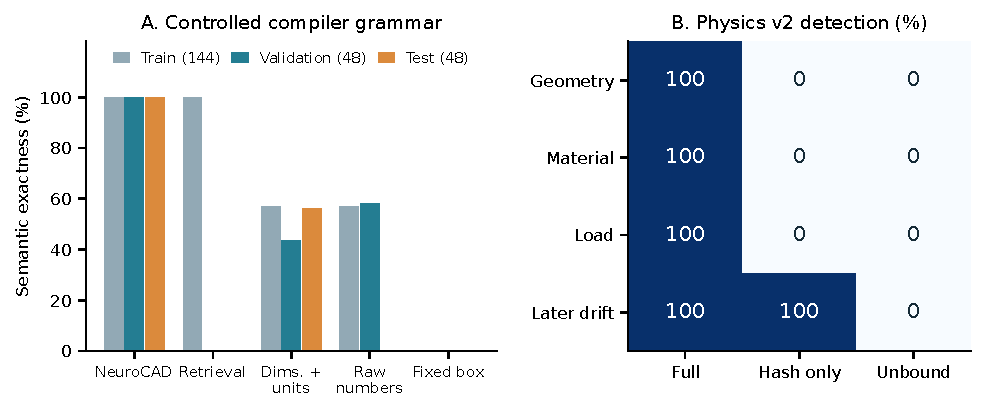
\includegraphics[width=\linewidth]{results_figure.pdf}
\caption{Retained results regenerated from raw records. Left: generated
compiler task exactness, with train/validation/test separation. Right: the
semantic-check versus content-freshness mechanism distinction in Physics v2.
No panel represents physical validation or a new model-training result.}
\label{fig:results}
\end{figure}

\subsection{Internal repetition outcome}

The hosted execution completed all 216 cases without recorded study execution
errors. All 13 endpoint definitions and counts match the original metrics.
For every case, the family, model, expected predicates, and applicable arm
outcomes for acceptance, detection, freshness, and repeated determinism match
the original raw records. The hosted ledger records \code{EXECUTED_ONCE}.
These observations support portability of the tested contract verdicts across
the two recorded environments. The raw records preserve verdicts and
within-run determinism flags, not complete numerical analytical reports;
cross-host bitwise equality of those numerical reports is not established.
The denominator remains 216 unique designed cases; counting the repeated
execution as an additional 216 independent observations would be incorrect.
Raw bytes, elapsed times, and path-dependent receipt identities need not
match across hosts. We make no cross-machine speed claim.

\subsection{Timing and a descriptive-statistic correction}

The frozen v2 report labels an upper-middle order statistic as the median for
even sample sizes. To preserve its identity, we retain that report unchanged
and state the convention here. Its successful-evaluation upper medians are
0.6185\,ms for full binding (\(n=120\)), 0.248\,ms for hash-only (\(n=192\)),
and 0.013209\,ms for unbound (\(n=216\)). The conventional average-of-two
middle values, re-read from the same raw records, are respectively
0.6178125, 0.2476455, and 0.0132085\,ms. The frozen upper-median full-report
size is 3,902 bytes; the conventional median is 3,763.5 bytes, with maximum
4,199 bytes. This diagnostic correction does not change a primary endpoint,
case outcome, or study disposition.

The uneven successful-only denominators are the more material efficiency
limitation. Rejecting a contradiction omits that arm from the timed sample;
the table is not a balanced cost comparison. No throughput, memory-scaling,
or optimized-compute benefit is established by these medians.

\section{Archival integrity and historical reconciliation}

The current read-only audit verifies every available file named by the
compiler manifest. Of 1,212 listed artifacts, 1,211 are present and match
their SHA-256 values. The listed \code{logs/run.log} is missing; no mismatched
present artifact is found. The numerical outcome records remain available,
but complete archival preservation cannot be claimed. The missing original
log is not recreated from a new execution.

The compiler's original \code{neurocad-deterministic-results-v1} digest also
contains ten timing values. Its hash identifies the recorded bytes, but is
not timing independent. A later format-v2 engineering repair separates those
fields from deterministic outcomes. The historical digest and study remain
unchanged. Together with the median convention above, these findings illustrate
why a hash-consistent artifact can still contain a misleading measurement
description.

Physics v2 has a separate retained freeze, execution ledger, raw JSONL,
metrics, and generated-result source. The present audit verifies their
recorded identities and confirms that regeneration of the existing result
source is byte-identical. This read-only reanalysis is separate from the
new hosted execution. The original environment is macOS ARM64 with Python
3.14.0; the repeated execution uses the archived source on Linux and Python
3.12.14. Neither the original run nor the internal repetition constitutes
independent external reproduction. No result is represented as Kaggle evidence.

Version routing matters. Historical narratives sometimes state that a feature
or release did not yet exist. Later engineering receipts can supersede a
product-status statement without revising a completed scientific result.
The published \code{v0.5.0a6} alpha and later native backend checks therefore
do not change the original mixed disposition or the v2 contract boundary.
The current repository state is an implementation successor, not the exact
source used in every historical experiment.

\section{Engineering successors and failure analysis}

\subsection{Physics v3 and exact geometry}

Physics v3 implements temperature-aware property cards, named load
combinations, cantilever mechanics, combined stress, linear thermal networks,
forced vibration, bounded pipe networks, and a lumped electro-thermal model.
It also provides corner enumeration, independent-uniform Monte Carlo, and
local finite-difference sensitivity wrappers. These are engineering
capabilities with stated assumptions, not additional v2 endpoints.

A retained v3 matrix originally passed 31/32 cases. Opposing beam loads
exposed an underestimated maximum bending stress: checking only the fixed
end gave zero while an interior moment extremum required 2.1\,MPa. The
versioned correction considers interior extrema and its known-case
successor reports 37/37 source scalar cases and 52/52 installed cases or
workflows. Since the failure was already observed, these are regression
conformance results. They do not transform into blinded confirmation when
the repaired cases pass.

Native acceptance and mesh-tagging records add backend-specific engineering
evidence. The 22 October feature IR scalar repair addresses malformed inputs
that could escape a structured parse error through operations such as hashing,
conversion, or unchecked comparison. Of 74 new authored regression cases,
the baseline failed 46 and passed 28. The repaired candidate passed 122
focused tests including existing feature/inspection coverage; a connected
suite passed 158 tests with five optional-backend skips. These overlapping
suites must not be summed as independent evidence. The repair improves the
admission boundary; it introduces no trained model and does not change the
frozen compiler or v2 scientific records.

\Needspace{10\baselineskip}
\subsection{What can still fail}

\begingroup
\small
\setlength{\tabcolsep}{4pt}
\begin{longtable}{>{\raggedright\arraybackslash}p{0.22\linewidth}>{\raggedright\arraybackslash}p{0.08\linewidth}>{\raggedright\arraybackslash}p{0.31\linewidth}>{\raggedright\arraybackslash}p{0.32\linewidth}}
\caption{Failure analysis and evidence required to close each gap.
Severity concerns the consequence for claims, not a measured incident rate.}
\label{tab:failure}\\
\toprule
Flaw and cause & Severity & Existing mitigation or justified change &
Required additional evidence \\
\midrule
\endfirsthead
\toprule
Flaw and cause & Severity & Existing mitigation or justified change &
Required additional evidence \\
\midrule
\endhead
\midrule
\multicolumn{4}{r}{\emph{Continued on next page}}\\
\endfoot
\bottomrule
\endlastfoot
Wrong intent passes: parser and reference share assumptions &
High & Explicit supported grammar, separate signatures, error records &
Independent prompt authors and adjudicators; false-acceptance analysis \\
Weak comparator: reduced feature vocabulary or memorization &
High & Report train and held-out labels separately; limit comparative claims &
Frozen grammar-independent comparator with matched task and retry budget \\
Stale calculation: geometry changed after evaluation &
High & Content hash and re-resolution for the selected component &
Broader adapters and consistent-read semantics for external systems \\
Wrong but current calculation: bad model or source declaration &
High & Assumptions and source fields retained; no physical certificate &
Qualified model selection, calibrated measurements, source governance \\
Partial mapping: hollow bore or boundary subset is unverified &
High & List exactly which quantities were checked &
Independent full-solid and boundary-condition reference checks \\
Numerical edge: overflow, Boolean coercion, cancellation &
High & Finite strict admission and case-specific numerical regressions &
Systematic domain-boundary tests and justified precision analysis \\
Hidden interior extremum: endpoint-only physics checks &
High & Retained beam failure and separately versioned correction &
Complete extremum conditions for each admitted load family \\
Corner envelope misses interior extrema &
High & Label corner enumeration as screening &
Monotonicity proof, rigorous interval method, or explicit interior search \\
Hash matches but archive is incomplete &
Medium & Report missing log and preserve original manifest &
Recovery of the original log, never a fabricated replacement \\
Timing diagnostic appears to prove efficiency &
Medium & State successful-only denominators and median convention &
Balanced instrumented successor with all attempted cases timed \\
Changing geometry loses edit intent &
High & Named parameters and semantic selector design &
History rebuild and relation-preservation benchmark; user observation \\
Manufactured fit or safety differs from software result &
High & Physical and usability gates remain open &
Calibrated physical measurements under a frozen study protocol \\
\end{longtable}
\endgroup

Table~\ref{tab:failure} makes the main remaining flaws concrete. An
uncertainty wrapper deserves particular care. Evaluating all \(2^d\) corners
of a bounded box gives a global range only under additional structural
conditions, such as suitable monotonicity; a nonlinear interior maximum can
be missed. Independent uniform Monte Carlo samples describe the declared
sampling model, not a calibrated real-world probability distribution.
Finite-difference sensitivities are local and can be inaccurate near
discontinuities, invalid domains, or poor step scales.

Material cards in the evaluated v2 contract are embedded declarations.
Only selected geometry has a freshness re-resolution API. External material
database changes and changing requirements are not automatically detected.
Whole-request hashes also include path text, so moving an otherwise
equivalent project may change request identity. Reproduction should distinguish
that from canonical geometry-content identity.

\section{Independent evaluation and falsification boundary}

The existing \code{NC-EXT-EVAL-V0} protocol is pre-outcome methodology. It
requires at least 160 independently authored prompts, including at least
120 valid and 40 reject cases, separately adjudicated references, frozen
source and scorer identities, and full retention of attempted outcomes.
Authors may use the public supported-scope documentation but not parser
internals or hidden failure cases. A strong grammar-independent comparator
is required for a comparative language-understanding claim. Valid semantic
exactness and fail-closed rejection are separate primary endpoints.

That external study is unexecuted in the evidence consolidated here.
Authoring more prompts after inspecting the code is useful development work,
but cannot satisfy its independence requirement. A new study must respect
the frozen boundary or explicitly become a different successor protocol.
No physical measurements or intended-user outcomes are supplied by
conformance tests, hosted CI, or the existence of a release package.

The strongest immediate falsifier for a claimed admission contract is an
in-scope input whose required semantic field is wrong while the system
accepts it. For freshness, it is a protected field change that remains
current; for specificity, a permitted non-geometric change that becomes
stale. For physical usefulness, these software counterexamples are
insufficient: the falsifier must be a measured failure of the prespecified
physical endpoint. The evidence needed depends on which claim is made.

\section{Discussion}

The positive results are useful because they identify narrow behavior that
has actually been exercised. Unit normalization, feature construction, static
checks, explicit dependency comparison, and artifact recording can be
combined into an inspectable pipeline. The ablations show a clear mechanistic
division: content identity detects changed content; semantic mapping checks
detect selected inconsistencies between current content and analytical inputs.
One cannot replace the other.

At the same time, complete success on a self-authored contract is partly
expected. A compiler is designed to implement its grammar, and a stored hash
is designed to change when the serialized content changes. The scientific
value lies in an exact specification, falsifiable failure cases, fair
accounting, and reproducibility, not in treating an expected conformance result
as broad evidence of intelligence or physical reliability.

The repaired system can be more useful without changing a completed study's
disposition. Separating successor implementation from predecessor evidence
prevents hindsight from making every historical version appear correct.
Keeping the wrong beam result, failed development run, missing log, and
typed-parser falsification visible is necessary to understand which
conclusions remain supported.

\section{Limitations, ethics, and reproducibility}

The central limits are author-generated data, restricted grammar and
representations, simple comparators, incomplete archive preservation, absence
of independent execution, and absence of physical or human evidence. This
paper does not report SOTA comparisons, fabrication qualification, safety
certification, or a learned-model contribution. A component-level scalar
annotation is not a finite-element stress field; an analytical pipe formula
is not CFD. The project should not present these different objects under
interchangeable labels.

The studied synthetic records contain no personal data. The practical concern
is overtrust: a reproducible and internally consistent CAD artifact can still
be unsuitable for its intended use. The appropriate response is precise
claim labeling and evidence appropriate to the intended application, rather
than interpreting a software pass as permission to manufacture.

The numerical result tables and the result figure are regenerated by
\path{paper/recovery_20261022/generate_evidence.py} from retained records.
It writes only this manuscript's derived outputs and a source-hash audit;
it launches no compiler, model, kernel, or protected study. The exact user
style file is copied unchanged into this source package. Appendix~\ref{app:evidence}
identifies authoritative records and reproduction commands. Code is in
\url{https://github.com/THE-BU1LD/NeuroCAD} under the repository's MIT license.
The scored data are repository-generated controlled fixtures; no dataset
from a cited CAD learning system is evaluated here. External kernels and
packaged third-party resources retain their respective licenses. This
document is a complete current-evidence manuscript,
not a claim that the independent external-validation program is complete.

\section{Conclusion}

NeuroCAD implements an inspectable bounded CAD compiler and an analytical
receipt mechanism. Retained compiler evidence establishes controlled
grammar and kernel conformance, while the separately frozen 216-case
receipt study supports its declared semantic-consistency and geometry-
freshness contract. One internal repetition reproduces its endpoint counts
on another environment, while independent confirmation remains open.
Present artifact auditing also identifies a missing
original log and diagnostic-description issues that must accompany those
results. The original study remains mixed and the historical typed-parser
claim remains falsified. Broader language validity, physical fit, and user
benefit require their own independent evidence; they have not been supplied
by the positive software outcomes reported here.

\bibliographystyle{plainnat}
\bibliography{references}

\appendix
\section{Mathematical and implementation details}

\subsection{Why hashing and semantic checking differ}

Consider a cylinder of radius \(r\) with recorded content hash \(h\). A
request can carry \(h\) correctly while specifying an outer diameter
\(D_o\ne2r\). Hash-only checking passes because the component has not changed;
the full arm rejects when the discrepancy exceeds
Eq.~\eqref{eq:geometrytol}. Conversely, changing the cylinder radius after a
valid calculation invalidates the stored content hash, even if the same
numeric analytical inputs remain syntactically well formed. These are
different predicates over different objects.

A label-only edit is deliberately excluded from canonical geometry. That
specificity prevents an irrelevant display change from invalidating the
calculation's geometry identity. It does not imply semantic equivalence of
every edit excluded by a future schema: exclusions need explicit review.
Hash collision resistance is an assumption about content addressing;
authenticating a signer would require a different mechanism.

\subsection{Selected v3 equations and assumption boundaries}

These formulas describe later engineering implementations and are not
additional outcomes of the v2 study. For a cantilever with constant \(EI\),
tip force \(F\), uniform load \(q\), and length \(L\), the linear tip response is
\begin{equation}
\delta(L)=\frac{FL^3}{3EI}+\frac{qL^4}{8EI},\qquad
\theta(L)=\frac{FL^2}{2EI}+\frac{qL^3}{6EI}.
\end{equation}
With opposing signed loads, maximum absolute bending moment must also inspect
admitted interior stationary points of
\(M(x)=F(L-x)+q(L-x)^2/2\), not only \(x=0\).
The physical assumptions remain linear small-deflection Euler--Bernoulli
behavior and the specified load family.

For a symmetric stress tensor \(\boldsymbol\sigma\), principal stresses are
its eigenvalues, hydrostatic stress is
\(\operatorname{tr}(\boldsymbol\sigma)/3\), and
\begin{equation}
\sigma_{\mathrm{VM}}=
\sqrt{\tfrac12[(\sigma_x-\sigma_y)^2+(\sigma_y-\sigma_z)^2+
(\sigma_z-\sigma_x)^2]+3(\tau_{xy}^2+\tau_{yz}^2+\tau_{zx}^2)}.
\end{equation}
This transforms a supplied local tensor; it does not solve for a spatial
stress field.

A linear thermal network solves conductance balance
\(\sum_j g_{ij}(T_i-T_j)=Q_i\) for free nodes with supplied fixed-temperature
nodes. Singular or invalid networks are rejected. For one linear forced mode,
the harmonic force amplitude response is
\begin{equation}
|X|=\frac{|F_0|}{\sqrt{(k-m\omega^2)^2+(c\omega)^2}},
\end{equation}
subject to the documented parameter and resonance checks. The electro-thermal
wire model assumes \(R=R_0(1+\alpha\Delta T)\) and
\(\Delta T=I^2R R_{\mathrm{th}}\), yielding
\begin{equation}
\Delta T=\frac{I^2R_0R_{\mathrm{th}}}
 {1-I^2R_0R_{\mathrm{th}}\alpha}.
\end{equation}
The implementation rejects feedback gain at least one. Uniform temperature,
constant thermal resistance, and the linear resistance law are assumptions,
not outcomes verified against experiment.

The uncertainty wrappers vary at most 12 supplied scalar inputs. Corner
enumeration uses \(2^d\) evaluations. Monte Carlo uses a declared seed,
independent uniform bounded draws, and 2--10,000 samples. Local sensitivity
uses central finite differences around the declared base point. None
automatically supplies missing physical parameter distributions.

\subsection{Statistical definitions}

For \(k\) successes among \(n\) fixed records, \(\hat p=k/n\). The reported
descriptive Wilson endpoints use \(z=1.9599639845\):
\begin{equation}
\frac{\hat p+z^2/(2n)\ \pm\
 z\sqrt{\hat p(1-\hat p)/n+z^2/(4n^2)}}{1+z^2/n}.
\end{equation}
For paired discordances \(b,c\), the exact two-sided McNemar diagnostic is
\begin{equation}
p=\min\left\{1,\ 2\sum_{j=0}^{\min(b,c)}
 \binom{b+c}{j}2^{-(b+c)}\right\}.
\end{equation}
When \((b,c)=(48,0)\), the result is \(2^{-47}\). Dependence among templates
or shared failure mechanisms prevents interpreting this calculation as
unqualified population evidence. No multiplicity-adjusted broad efficacy
claim is made; the primary deterministic decision rule is an all-cases
contract threshold.

For sorted even-\(n\) samples \(u_{(1)}\le\cdots\le u_{(n)}\), the frozen
diagnostic uses \(u_{(n/2+1)}\), whereas the conventional median is
\((u_{(n/2)}+u_{(n/2+1)})/2\). Disclosing the distinction is essential for
the receipt-size diagnostic because the middle two sizes differ materially.

\Needspace{10\baselineskip}
\section{Evidence map and reproduction}
\label{app:evidence}

\begin{longtable}{>{\raggedright\arraybackslash}p{0.22\linewidth}>{\raggedright\arraybackslash}p{0.72\linewidth}}
\caption{Repository-relative evidence map. Paths are versioned records, not
claims that every historical source matches the current checkout.}
\label{tab:evidence}\\
\toprule
Claim or boundary & Authoritative record \\
\midrule
\endfirsthead
\toprule Claim or boundary & Authoritative record \\
\midrule
\endhead
Original terminal status &
\path{TERMINAL_STATUS_2026-10-11.md}; \path{RESEARCH_TRUTH.md} \\
Compiler raw outcomes &
\path{research/runs/NC-REPRO-508EC40/metrics/results.json} \\
Compiler artifact manifest &
\path{research/runs/NC-REPRO-508EC40/manifest.json} \\
Compiler missing-log/digest erratum &
\path{docs/RESEARCH_PROVENANCE_AUDIT_20261014.md} \\
External study boundary &
\path{research/protocols/EXTERNAL_EVALUATION_V0.md} \\
Physics v2 specification &
\path{research/physics_v2/MODEL_SPEC.md};
\path{research/physics_v2/PROTOCOL.md} \\
Physics v2 freeze &
\path{research/physics_v2/frozen/freeze.json} \\
Physics v2 execution ledger &
\path{research/physics_v2/CONFIRMATORY_EXECUTION.json} \\
Physics v2 raw outcomes &
\path{research/physics_v2/runs/NC-PHYS-V2-CONFIRM-001/raw_results.jsonl} \\
Physics v2 analysis &
\path{research/physics_v2/runs/NC-PHYS-V2-CONFIRM-001/metrics.json};
\path{research/physics_v2/audit_results.py} \\
V3 negative conformance &
\path{docs/verification/physics-v3-20261014/REPORT.md} \\
V3 known-case repair &
\path{docs/verification/physics-v3-corrected-20261014/REPORT.md} \\
Current derived tables/figure &
\path{paper/recovery_20261022/generate_evidence.py};
\path{paper/recovery_20261022/evidence_sources.json} \\
Current separate reanalysis &
\path{research/recovery_20261022/evidence_reanalysis.json} \\
Internal v2 repetition &
\path{research/recovery_20261022/hosted-reproduction/declaration.json};
\path{research/recovery_20261022/hosted-reproduction/run/} \\
Repetition integrity audit &
\path{research/recovery_20261022/hosted_reproduction_audit.json} \\
Current engineering repair &
\path{research/recovery_20261022/engineering/} \\
Current full-suite execution &
\path{research/recovery_20261022/engineering/full-tests-with-sockets.txt};
\path{research/recovery_20261022/engineering/full-tests.txt} \\
Current native demonstration &
\path{research/recovery_20261022/native-demo/DEMO_RECEIPT.json} \\
\bottomrule
\end{longtable}

Important v2 identities are retained explicitly:
\begin{itemize}
\item Frozen source commit:
\path{2627c106ede6c2ac4e3570700f2bd545a763943c}.
\item Execution commit:
\path{786ba9ba5c2249a710529c3b07bf82d4e29c7f36}.
\item Frozen cases SHA-256:
\path{9caa80fb7e5257f514143ec0b297711464767c5a68ffa49988070a2f97c94c49}.
\item Raw outcomes SHA-256:
\path{97bae6a791a16088d4b9902ccc45fd0f291751d3dde822f7fad5c21c4add9023}.
\item Metrics SHA-256:
\path{34bb77ddf92225a4ee85e5c3f2a67dbca74c1cda23f60e3c9548ddf3fb013573}.
\end{itemize}
Hashes detect content differences relative to those records; they do not
authenticate an execution witness. The table/figure generator records fresh
hashes for every retained input it uses.

\paragraph{Current native demonstration.}
A separate 22 October engineering demonstration produced 32 hash-listed
artifacts through OpenSCAD 2021.01, including plate, cylinder, and enclosure
body/lid geometry. It also rejected the unsupported request to design a
load-rated aircraft engine mount. The version-2 demo receipt obtains producer
identity from the selected NeuroCAD CLI before and after execution, and the
two identities match. Its identity scope covers on-disk project sources and
packaged resources; it excludes loaded bytecode and third-party dependencies.
The observed checkout revision is explicitly not treated as verification of
the modified implementation. Physical validation is recorded as not performed.
These native artifact results supplement engineering reproducibility without
adding compiler benchmark cases or physics-study endpoints.

The maintained current-source suite passed 2,240 tests with 12 skips and
53 reported subtest passes under Python 3.12.14 in 98.32 seconds. An initial
sandboxed run retained 2,208 passes, 13 skips, four failures, and 27 errors;
all 31 failures/errors were socket-permission failures. The successful
rerun enabled local test-server sockets without weakening code or tests.
Both logs are retained under the engineering evidence directory. Suite,
subtest, and focused-regression counts overlap and are not independent
scientific sample sizes.

\paragraph{Regenerate this manuscript only.}
From the repository root:
\begin{Verbatim}[fontsize=\small]
python paper/recovery_20261022/generate_evidence.py
cd paper/recovery_20261022
pdflatex -interaction=nonstopmode -halt-on-error main.tex
bibtex main
pdflatex -interaction=nonstopmode -halt-on-error main.tex
pdflatex -interaction=nonstopmode -halt-on-error main.tex
\end{Verbatim}
Python requires Matplotlib and NumPy for the derived figure. LaTeX requires
the included unchanged \code{arxiv.sty} and the packages declared in
\code{main.tex}. PDF compilation is separate from scientific execution.

\paragraph{Read-only compiler archive check.}
\begin{Verbatim}[fontsize=\small]
python scripts/audit_retained_artifacts.py \
  research/runs/NC-REPRO-508EC40/manifest.json
\end{Verbatim}
The presently missing original log means this audit returns failure for full
archival completeness. That is the expected disclosure, not a command to
repair or overwrite the archive.

\paragraph{Scientific reproduction.}
The original compiler uses its source-pinned reproduction procedure and
native OpenSCAD dependency. Physics v2's independent reproduction instructions
are in \path{research/physics_v2/EXTERNAL_REPRODUCTION.md}; its completed
single-attempt confirmatory directory must not be reused. A legitimate
independent reproduction is a separately identified run with its own
environment and output records. It does not mutate the original ledger or
become a second attempt to rescue the original hypothesis. In the present
session, the local v2 preflight was blocked by the frozen runner's 2-GiB
free-disk requirement; it did not launch the cases locally. The subsequent
internal hosted repetition is separately recorded at
\url{https://github.com/THE-BU1LD/NeuroCAD/actions/runs/39726824693}.
Its workflow revision is
\path{95aa315e87e0546191bbcdbce60f9c083b43b4b6}; the evaluated source remains
\path{786ba9ba5c2249a710529c3b07bf82d4e29c7f36}.
The retrieved artifact archive has SHA-256
\path{4c8c9e7af18fcaed4a88d3ecd0bfa00d9b5161ae898ee20c7840d17e2220d217}.
The frozen JSONL file hash and the runner's canonical parsed-case digest
refer to different byte representations and must not be compared as if
they were the same hashing contract.

\paragraph{Release boundary.}
This manuscript and its source are a new synthesis package. No predecessor
paper, frozen protocol, dataset, run directory, or release tag is replaced.
No arXiv submission, external review, or independent participant contribution
is implied by compiling a PDF.

\end{document}
